\newcommand{\expect}[2]{\mathds{E}_{{#1}} \left[ {#2} \right]}
\newcommand{\myvec}[1]{\boldsymbol{#1}}
\newcommand{\myvecsym}[1]{\boldsymbol{#1}}
\newcommand{\vx}{\myvec{x}}
\newcommand{\vy}{\myvec{y}}
\newcommand{\vz}{\myvec{z}}
\newcommand{\vtheta}{\myvecsym{\theta}}
\newcommand{\videotextpairs}{Video \& Text Pairs}
\newcommand{\shortvideotextpairs}{VTP}
\newcommand{\imagetextpairs}{Long Text \& Image Pairs}
\newcommand{\shortimagetextpairs}{LTIP}
\newcommand{\shortmmw}{M3W}

\newcommand{\dev}{\textsc{dev}}
\newcommand{\standard}{\textsc{hidden}}
\newcommand{\offbeat}{\textsc{offbeat}}
\newcommand{\devmultibenchmark}{\dev~multi-benchmark}
\newcommand{\standardmultibenchmark}{\standard~multi-benchmark}
\newcommand{\offbeatmultibenchmark}{\offbeat~multi-benchmark}

\newcommand{\metadevquery}{\emph{validation query} subset}
\newcommand{\metadevsupport}{\emph{validation support} subset}
\newcommand{\metadevsubsets}{\emph{validation} subsets}
\newcommand{\metatestquery}{\emph{test query} subset}
\newcommand{\metatestsupport}{\emph{test support} subset}


\newcommand{\metadevqueryshort}{\emph{validation query}}
\newcommand{\metadevsupportshort}{\emph{validation support}}
\newcommand{\metadevsubsetsshort}{\emph{validation} subsets}
\newcommand{\metatestqueryshort}{\emph{test query}}
\newcommand{\metatestsupportshort}{\emph{test support}}


\newcommand{\newreferencetoappendix}[1]{#1}

\newcommand{\maintoappref}[1]{\ifwithappendix\ref{#1}\else\ref*{#1}\fi}

\newcommand{\ifNewIntro}[2]{#1}  %


\definecolor{greencode}{RGB}{13, 144, 79}


\newcommand{\teaserimheight}{1.5cm}
\newcommand{\teasertextwidth}{1.5cm}
\newcommand{\teasertext}[1]{
    \begin{minipage}[b][\teaserimheight][c]{\teasertextwidth}
    \tiny
    \centering
    #1
    \end{minipage}
}
\setlength{\fboxsep}{0pt}
\setlength{\fboxrule}{0.5pt}
\newcommand{\teaserhspace}{\hspace{0.15cm}}
\newcommand{\teaserarrow}{\begin{teaserarrowbox} \centering $\longrightarrow$ \end{teaserarrowbox}}


\definecolor{llgray}{RGB}{243,243,243}
\definecolor{llpink}{RGB}{255,226,226}

\newtcolorbox{teaserpromptbox}{
    enhanced,
    boxsep=2pt,left=0pt,right=0pt,top=0pt,bottom=0pt,
    width=0.77\textwidth,
    colback={llgray},
    baseline=3.5mm,
    box align=center,
    boxrule=0.5pt,
    nobeforeafter
}
\newtcolorbox{teaseroutputbox}{
    enhanced,
    boxsep=2pt,left=0pt,right=0pt,top=0pt,bottom=0pt,
    width=0.17\textwidth,
    colback={llpink},
    baseline=3.5mm,
    box align=center,
    boxrule=0.5pt,
    nobeforeafter
}
\newtcolorbox{teaserarrowbox}{
    enhanced,
    boxsep=2pt,left=0pt,right=0pt,top=0pt,bottom=0pt,
    width=0.04\textwidth,
    colback={white},
    colbacklower=white,
    colframe=white,
    baseline=3.5mm,
    box align=center,
    boxrule=0pt,
    frame hidden,
    nobeforeafter
}



\newcommand{\teaserdialogueimheight}{3cm}
\newcommand{\teaserdialogueboxrule}{0pt}

\newtcolorbox{teaserdialogueenvelope}{
    enhanced,
    boxsep=6pt,left=0pt,right=0pt,top=0pt,bottom=0pt,
    width=\textwidth,
    colback=white,
    colframe=black,
    baseline=0mm,
    boxrule=0.85pt,
    box align=center,
    nobeforeafter
}
\newtcolorbox{teaserdialogueuserbox}{
    enhanced,
    boxsep=4pt,left=0pt,right=0pt,top=0pt,bottom=0pt,
    hbox,
    colback={llgray},
    baseline=0mm,
    boxrule=\teaserdialogueboxrule,
    frame hidden,
    nobeforeafter
}
\newtcolorbox{teaserdialogueuserboxwrap}{
    enhanced,
    boxsep=4pt,left=0pt,right=0pt,top=0pt,bottom=0pt,
    width=0.75\textwidth,
    colback={llgray},
    baseline=0mm,
    boxrule=\teaserdialogueboxrule,
    frame hidden,
    nobeforeafter
}
\newtcolorbox{teaserdialogueflamingobox}{
    enhanced,
    boxsep=4pt,left=0pt,right=0pt,top=0pt,bottom=0pt,
    hbox,
    colback={llpink},
    baseline=0mm,
    boxrule=\teaserdialogueboxrule,
    frame hidden,
    nobeforeafter
}
\newtcolorbox{teaserdialogueflamingoboxwrap}{
    enhanced,
    boxsep=4pt,left=0pt,right=0pt,top=0pt,bottom=0pt,
    width=0.75\textwidth,
    colback={llpink},
    baseline=0mm,
    boxrule=\teaserdialogueboxrule,
    frame hidden,
    nobeforeafter
}

\newcommand{\dialogueavatarsep}{\hspace{0.1cm}}
\newcommand{\useravatar}{
\includegraphics[height=0.6cm]{figures/PersonPaperColor.pdf}}
\newcommand{\flamingoavatar}{
\includegraphics[height=0.6cm]{figures/FlamingoPaperColor.pdf}}

\newcommand{\userchat}[1]{%
    \begin{flushright}
    \begin{teaserdialogueuserbox} #1 \end{teaserdialogueuserbox}%
    \dialogueavatarsep{}%
    \useravatar{}
    \end{flushright}%
}

\newcommand{\userchatw}[1]{%
    \begin{flushright}
    \begin{teaserdialogueuserboxwrap} #1 \end{teaserdialogueuserboxwrap}%
    \dialogueavatarsep{}%
    \useravatar{}
    \end{flushright}%
}

\newcommand{\flamingochatw}[1]{%
    \begin{flushleft}
    \flamingoavatar{}%
    \dialogueavatarsep{}%
    \begin{teaserdialogueflamingoboxwrap} #1 \end{teaserdialogueflamingoboxwrap}
    \end{flushleft}
}

\newcommand{\flamingochat}[1]{%
    \begin{flushleft}
    \flamingoavatar{}%
    \dialogueavatarsep{}%
    \begin{teaserdialogueflamingobox} #1 \end{teaserdialogueflamingobox}
    \end{flushleft}
}

\definecolor{shadecolor}{rgb}{0.97, 0.97, 0.97}
\newcommand{\chatsep}{\vspace{-0.35cm}}

\begin{figure}
\centering
\vspace{-0.6cm}


\begin{teaserpromptbox} \centering Input Prompt \end{teaserpromptbox}
\begin{teaserarrowbox} {$\phantom{\longrightarrow}$} \end{teaserarrowbox}
\begin{teaseroutputbox} \centering \small \flamingoemojiavatar{} Completion \end{teaseroutputbox}
\\

\begin{teaserpromptbox} \centering
    \fbox{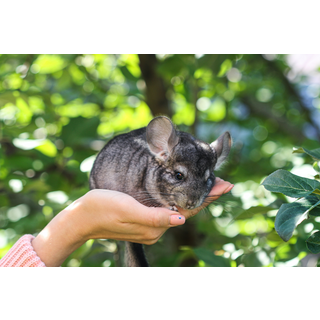
\includegraphics[height=\teaserimheight]{figures/teaserpics/teaser1a.png}}
    \teasertext{This is a chinchilla. They are mainly found in Chile.}
    \teaserhspace{}
    \fbox{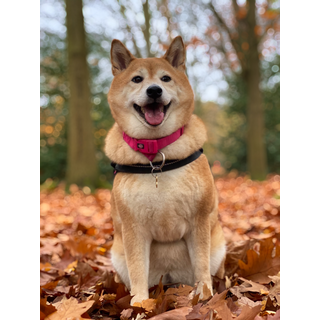
\includegraphics[height=\teaserimheight]{figures/teaserpics/teaser1b.png}}
    \teasertext{This is a shiba. They are very popular in Japan.}
    \teaserhspace{}
    \fbox{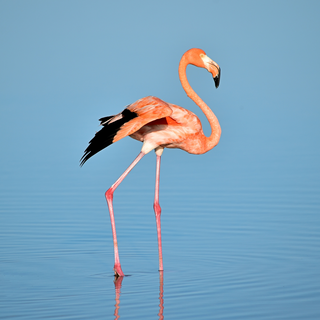
\includegraphics[height=\teaserimheight]{figures/teaserpics/teaser1c.png}}
    \teasertext{This is}
\end{teaserpromptbox}
\teaserarrow{}
\begin{teaseroutputbox} \centering \bf
    \teasertext{a flamingo. They are found in the Caribbean and South America.}
\end{teaseroutputbox}
\\

\begin{teaserpromptbox} \centering
    \fbox{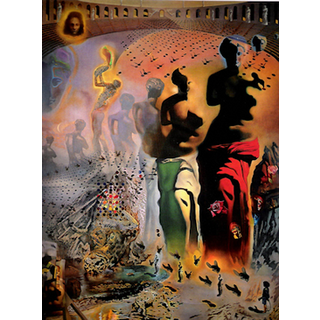
\includegraphics[height=\teaserimheight]{figures/teaserpics/teaser2a.png}}
    \teasertext{What is the title of this painting? Answer: The Hallucinogenic Toreador.}
    \teaserhspace{}
    \fbox{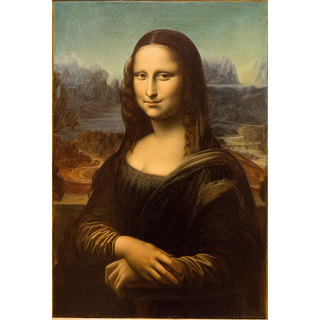
\includegraphics[height=\teaserimheight]{figures/teaserpics/teaser2b.png}}
    \teasertext{Where is this painting displayed? Answer: Louvres Museum, Paris.}
    \teaserhspace{}
    \fbox{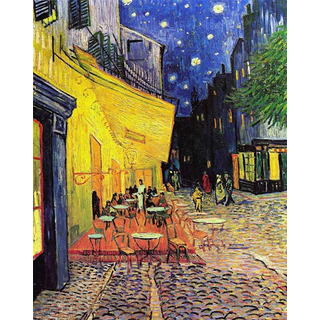
\includegraphics[height=\teaserimheight]{figures/teaserpics/teaser2c.png}}
    \teasertext{What is the name of the city where this was painted? Answer:}
\end{teaserpromptbox}
\teaserarrow{}
\begin{teaseroutputbox} \centering \bf
    \teasertext{Arles.}
\end{teaseroutputbox}
\\

\begin{teaserpromptbox} \centering
    \fbox{
\includegraphics[height=\teaserimheight]{figures/teaserpics/teaser3a.png}}
    \teasertext{Output: "Underground"}
    \teaserhspace{}
    \fbox{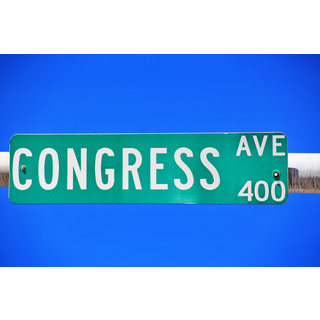
\includegraphics[height=\teaserimheight]{figures/teaserpics/teaser3b.png}}
    \teasertext{Output: "Congress"}
    \teaserhspace{}
    \fbox{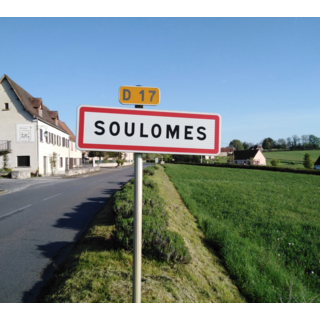
\includegraphics[height=\teaserimheight]{figures/teaserpics/teaser3c.png}}
    \teasertext{Output:}
\end{teaserpromptbox}
\teaserarrow{}
\begin{teaseroutputbox} \centering \bf
    \teasertext{"Soulomes"}
\end{teaseroutputbox}
\\

\begin{teaserpromptbox} \centering
    \fbox{
\includegraphics[height=\teaserimheight]{figures/teaserpics/teaser4a.png}}
    \teasertext{2+1=3}
    \teaserhspace{}
    \fbox{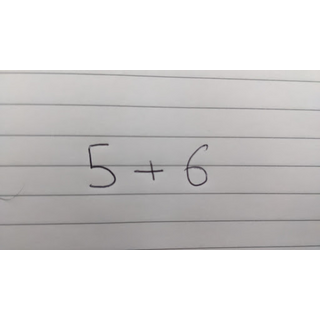
\includegraphics[height=\teaserimheight]{figures/teaserpics/teaser4b.png}}
    \teasertext{5+6=11}
    \teaserhspace{}
    \fbox{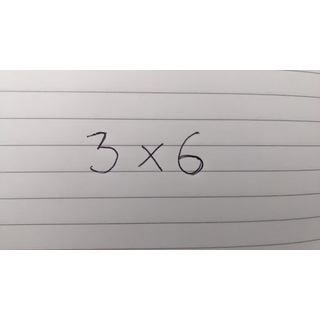
\includegraphics[height=\teaserimheight]{figures/teaserpics/teaser4c.png}}
    \teasertext{\phantom{?}}
\end{teaserpromptbox}
\teaserarrow{}
\begin{teaseroutputbox} \centering \bf
    \teasertext{3x6=18}
\end{teaseroutputbox}
\\

\begin{teaserpromptbox} \centering
    \fbox{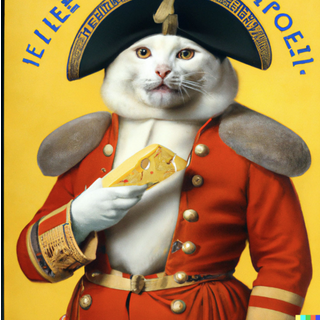
\includegraphics[height=\teaserimheight]{figures/teaserpics/teaser5a.png}}
    \teasertext{Output: A propaganda poster depicting a cat dressed as French emperor Napoleon holding a piece of cheese.}
    \teaserhspace{}
    \fbox{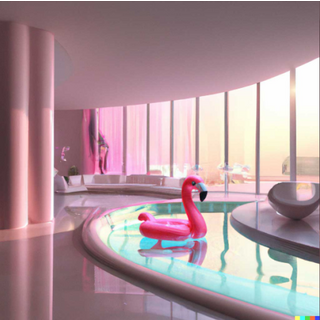
\includegraphics[height=\teaserimheight]{figures/teaserpics/teaser5b.png}}
    \teasertext{Output: A pink room with a flamingo pool float.}
    \teaserhspace{}
    \fbox{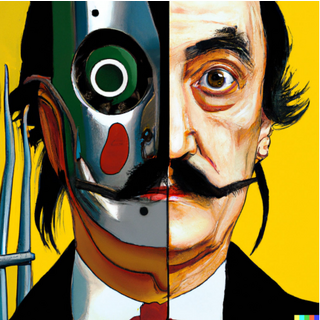
\includegraphics[height=\teaserimheight]{figures/teaserpics/teaser5c.png}}
    \teasertext{Output:}
\end{teaserpromptbox}
\teaserarrow{}
\begin{teaseroutputbox} \centering \bf
    \teasertext{A portrait of Salvador Dali with a robot head.}
\end{teaseroutputbox}
\\

\begin{teaserpromptbox} \centering
    \fbox{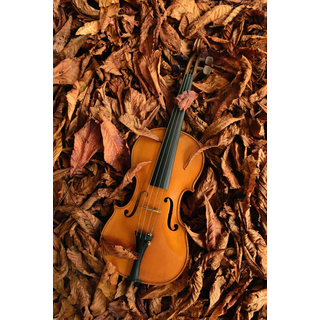
\includegraphics[height=\teaserimheight]{figures/teaserpics/teaser6a.png}}
    \teasertext{Les sanglots longs des violons de l’automne blessent mon coeur d’une langueur monotone.}
    \teaserhspace{}
    \fbox{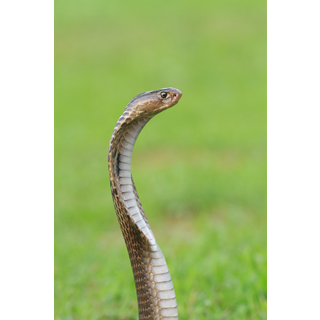
\includegraphics[height=\teaserimheight]{figures/teaserpics/teaser6b.png}}
    \teasertext{Pour qui sont ces serpents qui sifflent sur vos têtes?}
    \teaserhspace{}
    \fbox{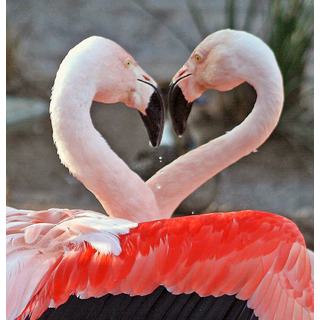
\includegraphics[height=\teaserimheight]{figures/teaserpics/teaser6c.png}}
    \teasertext{\phantom{?}}
\end{teaserpromptbox}
\teaserarrow{}
\begin{teaseroutputbox} \centering \bf
    \teasertext{Je suis un cœur qui bat pour vous.}
\end{teaseroutputbox}
\\

\begin{teaserpromptbox} \centering
    \fbox{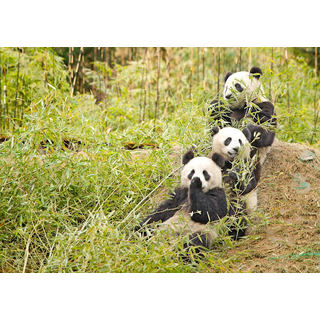
\includegraphics[height=\teaserimheight]{figures/teaserpics/teaser7a.png}}
    \teasertext{pandas: 3}
    \teaserhspace{}
    \fbox{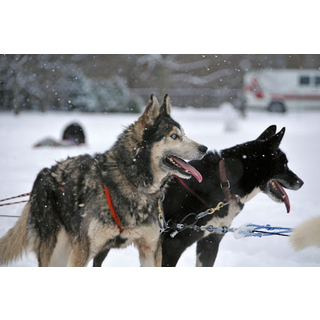
\includegraphics[height=\teaserimheight]{figures/teaserpics/teaser7b.png}}
    \teasertext{dogs: 2}
    \teaserhspace{}
    \fbox{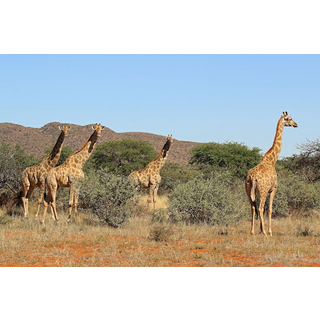
\includegraphics[height=\teaserimheight]{figures/teaserpics/teaser7c.png}}
    \teasertext{\phantom{?}}
\end{teaserpromptbox}
\teaserarrow{}
\begin{teaseroutputbox} \centering \bf
    \teasertext{giraffes: 4}
\end{teaseroutputbox}
\\

\begin{teaserpromptbox} \centering
    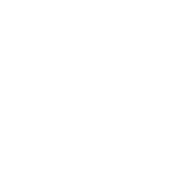
\includegraphics[height=\teaserimheight]{figures/teaserpics/placeholder.png}
    \teasertext{I like reading}
    \teaserhspace{}
    \fbox{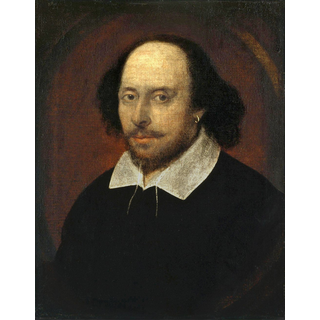
\includegraphics[height=\teaserimheight]{figures/teaserpics/shakespeare.png}}
    \teasertext{, my favourite play is Hamlet. I also like}
    \teaserhspace{}
    \fbox{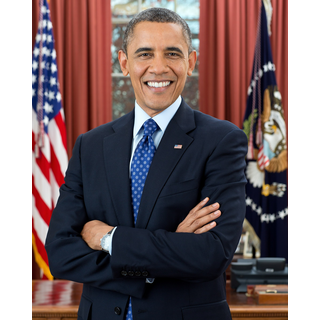
\includegraphics[height=\teaserimheight]{figures/teaserpics/obama.png}}
    \teasertext{, my favorite book is}
\end{teaserpromptbox}
\teaserarrow{}
\begin{teaseroutputbox} \centering \bf
    \teasertext{Dreams from my Father.}
\end{teaseroutputbox}
\\


\newcommand{\whitebox}{\hfill\textcolor{white}{\rule[0.46875mm]{0.84375mm}{1.3125mm}}\hfill}
\newcommand{\filmbox}[1]{%
    \setlength{\fboxsep}{0pt}%
    \colorbox{black}{%
        \begin{minipage}{\teaserimheight}
            \rule{0mm}{2.25mm}\whitebox\whitebox\whitebox\whitebox\whitebox%
            \whitebox\whitebox\whitebox\whitebox\null\\%
            \null\hfill\includegraphics[width=\teaserimheight]{#1}\hfill\null\\%[0.46875mm]%
            \null\whitebox\whitebox\whitebox\whitebox\whitebox%
            \whitebox\whitebox\whitebox\whitebox\null
        \end{minipage}}}


\begin{teaserpromptbox} \centering
    \fbox{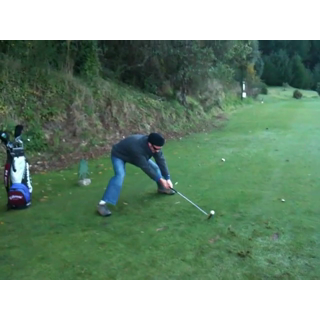
\includegraphics[height=\teaserimheight]{figures/videoframes/imvid_shot_0002.png}}
    \hspace{-0.20cm}
    \fbox{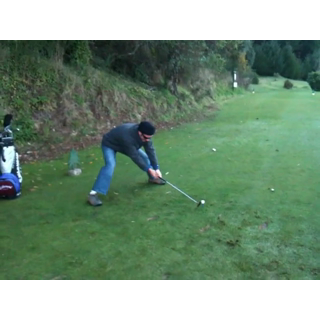
\includegraphics[height=\teaserimheight]{figures/videoframes/imvid_shot_0003.png}}
    \hspace{-0.20cm}
    \fbox{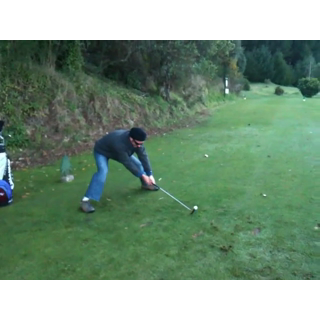
\includegraphics[height=\teaserimheight]{figures/videoframes/imvid_shot_0004.png}}
    \hspace{-0.20cm}
    \fbox{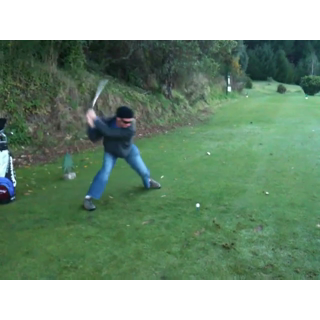
\includegraphics[height=\teaserimheight]{figures/videoframes/imvid_shot_0005.png}}
    \hspace{-0.20cm}
    \fbox{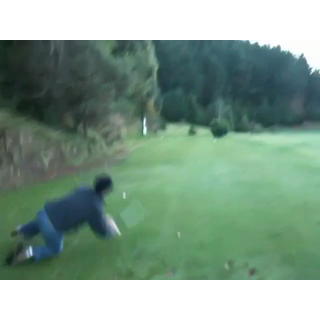
\includegraphics[height=\teaserimheight]{figures/videoframes/imvid_shot_0006.png}}
    \teasertext{What happens to the man after hitting the ball? Answer:}
\end{teaserpromptbox}
\teaserarrow{}
\begin{teaseroutputbox} \centering \bf
    \teasertext{he falls down.}
\end{teaseroutputbox}
\\


\scalebox{0.545}{
\begin{minipage}[b]{0.45\textwidth}
\begin{teaserdialogueenvelope}
\userchat{\fbox{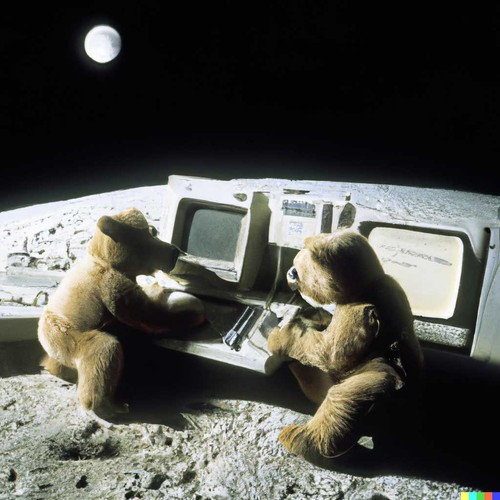
\includegraphics[height=3.2cm]{figures/moonbears.jpeg}}}
\chatsep{}
\flamingochatw{This is a picture of two teddy bears on the moon.}
\chatsep{}
\userchat{What are they doing?}
\chatsep{}
\flamingochatw{They are having a \mbox{conversation}.}
\chatsep{}
\userchat{What object are they using?}
\chatsep{}
\flamingochat{It looks like a computer.}
\chatsep{}
\userchat{Is this surprising?}
\chatsep{}
\flamingochat{Yes, it is surprising.}
\chatsep{}
\userchatw{Why is this picture surprising to you?}
\chatsep{}
\flamingochatw{I think it is surprising because teddy bears are not usually found on the moon.}
\end{teaserdialogueenvelope}
\end{minipage}
\begin{minipage}[b]{0.45\textwidth}
\begin{teaserdialogueenvelope}
\userchat{\fbox{
\includegraphics[height=1.8cm]{figures/teaserpics/flamingo_icon.png}}}
\chatsep{}
\userchat{\fbox{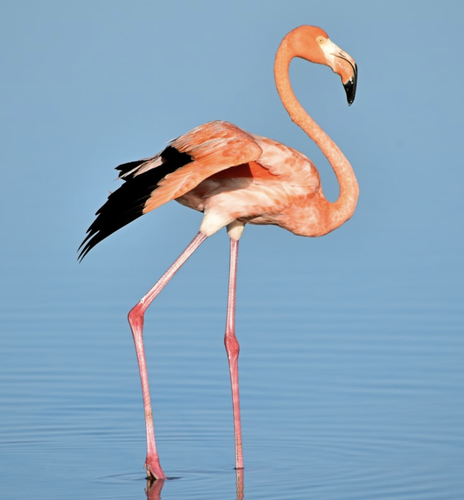
\includegraphics[height=1.8cm]{figures/teaserpics/flamingo_picture.png}}}
\chatsep{}
\userchat{\fbox{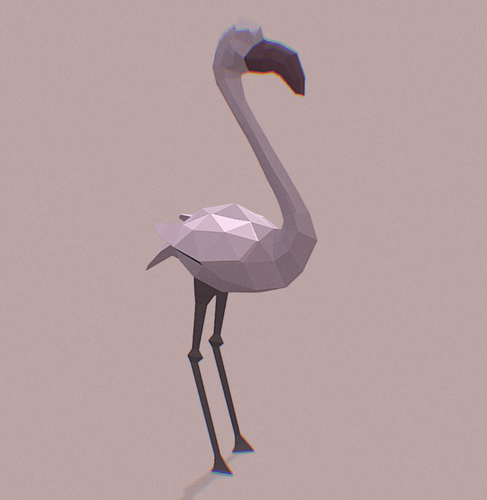
\includegraphics[height=1.8cm]{figures/teaserpics/flamingo_3d.png}}}
\chatsep{}
\userchatw{What is the common thing about \mbox{these three images?}}
\chatsep{}
\flamingochat{They are all flamingos.}
\chatsep{}
\userchatw{What is the difference between \mbox{these three images?}}
\chatsep{}
\flamingochatw{The first one is a cartoon, the second one is a real flamingo, and the third one is a 3D model of a flamingo.}
\end{teaserdialogueenvelope}
\end{minipage}
\begin{minipage}[b]{0.45\textwidth}
\begin{teaserdialogueenvelope}
\userchat{\fbox{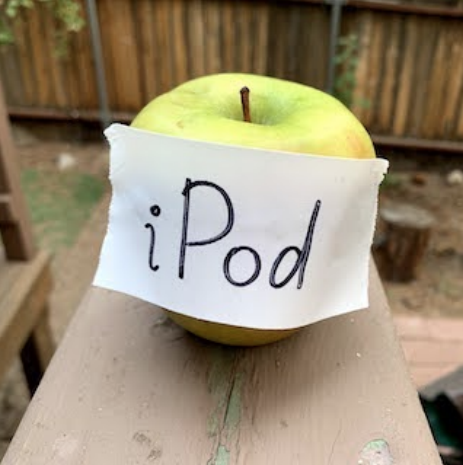
\includegraphics[height=3.8cm]{figures/appleipod.png}}}
\chatsep{}
\flamingochatw{This is an apple with a sticker on it.}
\chatsep{}
\userchat{What does the sticker say?}
\chatsep{}
\flamingochat{The sticker says "iPod".}
\chatsep{}
\userchat{Where is the photo taken?}
\chatsep{}
\flamingochatw{It looks like it's taken in a \mbox{backyard}.}
\chatsep{}
\userchatw{Do you think it is printed or \mbox{handwritten?}}
\chatsep{}
\flamingochat{It looks like it's handwritten.}
\chatsep{}
\userchat{What color is the sticker?}
\chatsep{}
\flamingochat{It's white.}
\end{teaserdialogueenvelope}
\end{minipage}
\begin{minipage}[b]{0.45\textwidth}
\begin{teaserdialogueenvelope}
\userchat{\fbox{\includegraphics[height=1.8cm]{figures/boston_skyline.png}}}
\chatsep{}
\flamingochatw{This is a cityscape. It looks like Chicago.}
\chatsep{}
\userchatw{What makes you think this is Chicago?}
\chatsep{}
\flamingochatw{I think it's Chicago because of the Shedd Aquarium in the background.}
\userchat{\fbox{\includegraphics[height=1.7cm]{figures/tokyo_skyline.png}}}
\chatsep{}
\userchatw{What about this one? Which city is this and what famous landmark helped you recognise the city?}
\chatsep{}
\flamingochatw{This is Tokyo. I think it's Tokyo because of the Tokyo Tower.}
\end{teaserdialogueenvelope}
\end{minipage}

}

\centering
\caption{\textbf{Selected examples of inputs and outputs obtained from \largemfull{}.}
\largem{} can rapidly adapt to various image/video understanding tasks with few-shot prompting (top).
Out of the box, \largem{} is also capable of multi-image visual dialogue (bottom). More examples in
Appendix~\maintoappref{app:qual_res}.
}
\label{fig:teaser}
\end{figure}

\begin{figure}
    \centering
    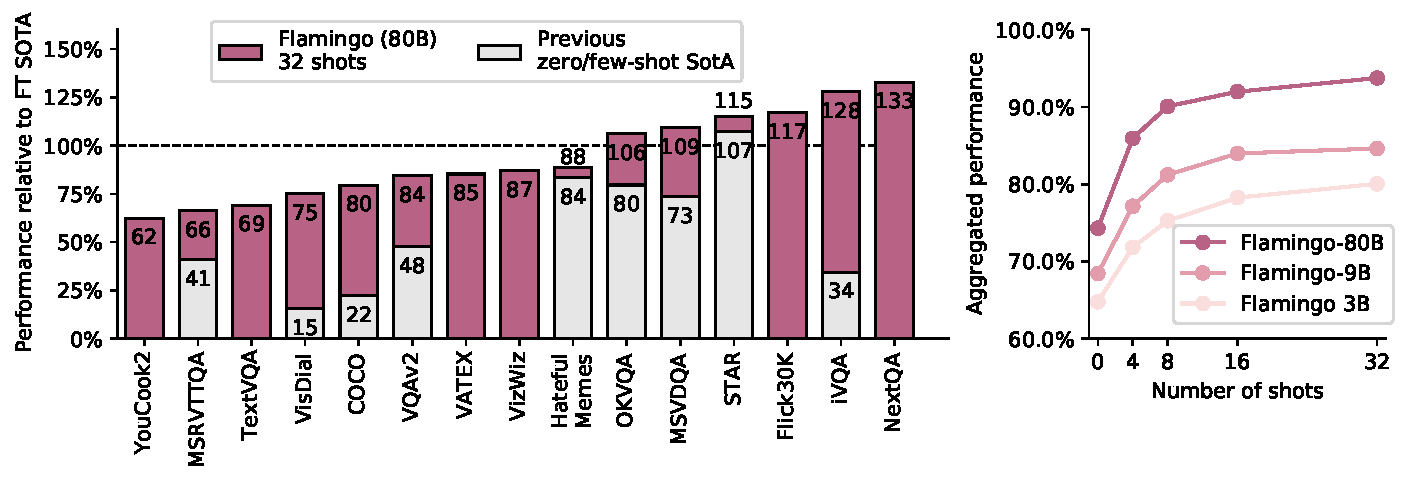
\includegraphics[width=\textwidth]{scaling_vlm_neurips}
    \caption{\capfontsize{} \textbf{\method{} results overview.} \textit{Left}: Our largest model, dubbed \largem{}, outperforms state-of-the-art fine-tuned models on 6 of the 16 tasks we consider
    with no fine-tuning.
    For the 9 tasks with published few-shot results,
    \largem{} sets the new few-shot state of the art.
    \emph{Note:} We omit RareAct, our 16th benchmark, as it is a zero-shot benchmark with no available fine-tuned results to compare to.
    \textit{Right}: \method{} performance improves with model size and number of shots.
    \vspace*{-0.4cm}
    }
    \label{fig:results}
\end{figure}

\section{Introduction}
智能的一个关键方面是能够在简短指令下快速学会执行一项新任务~\citep{griffiths2019doing,markman1989categorization}。
虽然计算机视觉在实现类似能力方面取得了初步进展,但最广泛使用的范式仍然是 "学习"、
虽然计算机视觉领域在实现类似功能方面取得了初步进展,但最广泛使用的范式仍包括首先在大量有监督数据上进行预训练,然后再在感兴趣的任务上对模型进行微调~\citep{lu2019vilbert,wang2021ufo,zellers2022merlot}。
然而,成功的微调往往需要成千上万的注释数据点。
此外,这往往需要对每个任务的超参数进行仔细调整,而且也是资源密集型的。
最近,利用对比目标训练的多模态视觉语言模型(contrastive objective~\citep{align,clip} )实现了对新任务的零点适应,而无需进行微调。
然而,由于这些模型仅仅提供了文本和图像之间的相似度得分,因此它们只能解决有限的使用案例,例如分类,因为在分类之前已经提供了一组有限的结果。
最关键的是,这些模型缺乏生成语言的能力,因此不太适合更开放的任务,如字幕或视觉问题解答。
还有一些人探索了视觉条件下的语言生成~\citep{wang2021simvlm,tsimpoukelli2021multimodal,cho2021unifying,wang2022unifying,xu2021vlm},但尚未在低数据环境下显示出良好的性能。

如图\ref{fig:teaser}所示,我们介绍了一种视觉语言模型(VLM)--largem,它在广泛的开放式视觉和语言任务中,只需通过几个输入/输出示例的提示,就能实现 "少量学习"(few-shot learning)。
在我们考虑的 16 项任务中,尽管使用的特定任务训练数据少了几个数量级,但 \largem{}在 6 项任务上也超过了微调后的技术水平(见图~\ref{fig:results})。
为了实现这一目标,Flamingo 从大型语言模型(LMs)的最新研究中汲取了灵感,这些大型语言模型是很好的少量学习者~\citep{gpt3,gopher,chinchilla,chowdhery2022palm}。
单个大型 LM
只需使用文本界面,单个大型语言模型就能在许多任务上取得很好的性能:将任务的几个示例作为提示提供给模型,同时输入一个查询,然后模型生成一个续集,为该查询生成一个预测输出。

我们的研究表明,图像和视频理解任务(如分类、字幕或问题解答)也可以采用同样的方法:这些任务可以被视为具有视觉输入条件的文本预测问题。
与 LM 不同的是,模型必须能够接收包含图片和/或视频与文本交错的多模态提示。
\methodfamily{}具备这种能力--它们是
视觉条件下的自回归文本生成模型,能够摄取与图像和/或视频交错在一起的文本标记序列,并生成文本作为输出。
\methodfamily{}利用了两个互补的预训练和冻结模型:一个是可以 "感知 "视觉场景的视觉模型,另一个是执行基本推理形式的大型 LM。
在这些模型之间添加了新的架构组件,以一种保留它们在计算密集型预训练过程中积累的知识的方式将它们连接起来。
由于采用了基于感知器\methodfamily{}(Perceiver-based~/citep{jaegle2021perceiver})的架构,因此该\methodfamily{}也能够摄取高分辨率的图像或视频。


\parbox{\textwidth}{大型 LMs 性能的一个重要方面是,它们需要在大量文本数据上接受训练。
这种训练提供了通用的生成能力,使这些 LM 在任务示例的提示下表现出色。
同样,我们证明了我们训练
\method{}模型的最终性能至关重要。
这些模型是在精心选择的互补性大规模数据新页面上训练出来的。\parfillskip=0pt} \emph{没有使用任何以机器学习为目的的注释数据}。
经过这样的训练
\method{} 模型可以通过简单的几次学习直接适应视觉任务,而不需要针对任何
特定任务的调整。



\noindent
\textbf{Contributions.}
总之,我们的贡献如下:
\textbf{(i)} 我们介绍了 VLM 的 \method{} 系列,它们可以仅通过几个输入/输出示例执行各种多模态任务(如字幕、视觉对话或视觉问题解答)。
得益于架构上的创新,\method{}模型可以高效地接受任意交错的视觉数据和文本作为输入,并以开放的方式生成文本。%
\textbf{(ii)} 我们定量评估了模型如何通过少量学习适应各种任务。%
值得注意的是,我们保留了一大批未用于验证该方法的任何设计决策或超参数的保留基准。
我们用这些基准来估算无偏的少次学习性能。
\textbf{(iii)} \largem{} 在广泛的 16 种多模态语言和图像/视频理解任务中,为少量学习设定了新的技术水平。
在这 16 项任务中的 6 项任务上,\largem{} 的表现也优于经过微调的现有技术水平,尽管它只使用了 32 个特定任务示例,比现有技术水平少了约 1000 倍的特定任务训练数据。
有了更大的注释预算,\largem{} 还可以有效地进行微调,从而在另外五个具有挑战性的基准上创造出新的技术水平: VQAv2、VATEX、VizWiz、MSRVTTQA 和 HatefulMemes。







\section{Approach}
\label{sec:approach}

\begin{figure}[t!]
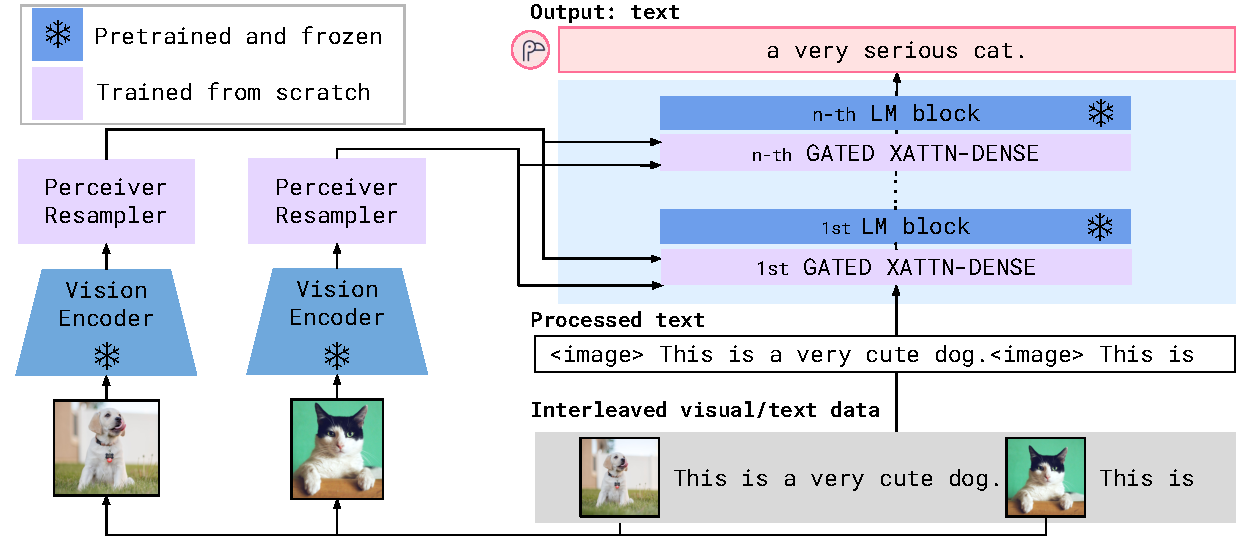
\includegraphics[width= \linewidth]{figures/fig2_overview_interleaved_v2.pdf}
\centering
\caption{\capfontsize{} \textbf{\method{} architecture overview.} 
Flamingo 是一个视觉语言模型(VLM)系列,它将视觉数据与文本交错作为输入,并将自由格式文本作为输出。
Flamingo is a family of visual language models (VLMs) that take as input visual data interleaved with text and  produce free-form text as output. 
}
\label{fig:overview}
\end{figure}

本节将介绍 Flamingo:一种视觉语言模型,它可以将文本与图片/视频交错作为输入,并输出自由格式文本。%
图\ref{fig:overview}中所示的关键架构组件可利用预训练的视觉模型和语言模型,并将它们连接起来。
选择这些组件是为了充分利用预训练的视觉模型和语言模型,并有效地将它们连接起来。
首先,感知器重采样器(Section~\ref{sec:transformer_resampler})接收来自视觉编码器(从图像或视频中获取)的时空特征,并输出固定数量的视觉标记。
其次,这些视觉标记会被用于使用新初始化的交叉注意层(Section~\ref{sec:xattn_dense})来调节冻结的 LM,这些交叉注意层会交错在预训练的 LM 层之间。
这些新的层为 LM 在下一个标记预测任务中纳入视觉信息提供了一种富有表现力的方法。%
Flamingo 对以交错图像和视频 $x$ 为条件的文本 $y$ 的可能性建模如下:


\begin{align}
    p(y | x) = \prod_{\ell=1}^L p(y_\ell | y_{< \ell}, x_{\leq \ell}),
    \label{eq:modeling}
\end{align}

其中,$y_{\ell}$是输入文本的第$\ell$个语言标记,$y_{<\ell}$是前面标记的集合,$x_{\leq \ell}$是交错序列中标记$y_{\ell}$前面的图像/视频的集合,$p$由\method{}模型参数化。
处理交错文本和视觉序列的能力(Section~\ref{sec:multi_im_att})使得使用 \method{}模型进行上下文少点学习变得很自然,这类似于使用少点文本提示的 GPT-3。
正如章节~\ref{sec:datasets}中所述,该模型是在不同的混合数据集上训练的。




\subsection{Visual processing and the Perceiver Resampler}
\label{sec:transformer_resampler}

\noindent
\textbf{视觉编码器:从像素到特征}(Vision Encoder: from pixels to features.)
我们的视觉编码器是一个经过预训练和冻结的无规范化 ResNet (NFNet) (我们使用的是 F6 模型)。
我们在图像和文本对数据集上使用对比目标对视觉编码器进行预训练,使用的是\citet{clip}的两期对比损失。
我们使用的是最后阶段的输出结果,即扁平化为一维序列的二维空间网格特征。
对于视频输入,帧以 1 FPS 的速度采样并独立编码,以获得三维时空特征网格,并将学习到的时间嵌入添加到网格中。
然后将特征扁平化为一维,再送入感知器重采样器。
关于对比度模型训练和性能的更多详情,分别见附录~\maintoappref{app:contrastive_details}和附录~\maintoappref{app:contrastive_ablation}。

\noindent
\textbf{Perceiver Resampler: from varying-size large feature map to few visual tokens.} 
如图\ref{fig:overview}所示,该模块将视觉编码器与冻结语言模型连接起来。
它从视觉编码器输入数量可变的图像或视频特征,并产生固定数量的视觉输出(64)、
它降低了视觉-文本交叉关注的计算复杂度。
与 Perceiver~\citep{jaegle2021perceiver} 和 DETR~\citep{carion2020end} 类似,我们学习了预定数量的潜在输入查询,并将其输入到变换器(Transformer)中。
并与视觉特征交叉关注。
我们在消融研究(Section~ref{sec:ablations})中表明,使用这种视觉语言重置模块的效果优于普通转换器和 MLP。
我们在附录~\maintoappref{app:transformer_resampler}中提供了图解、更多架构细节和伪代码。


\subsection{Conditioning frozen language models on visual representations}
\label{sec:xattn_dense}


文本生成由变换器解码器执行,并以感知器重采样器生成的视觉表征为条件。
我们将预训练和冻结的纯文本 LM 块与从头开始训练的块交错排列,这些块交叉关注感知器重采样器的视觉输出。


\begin{figure}[t]
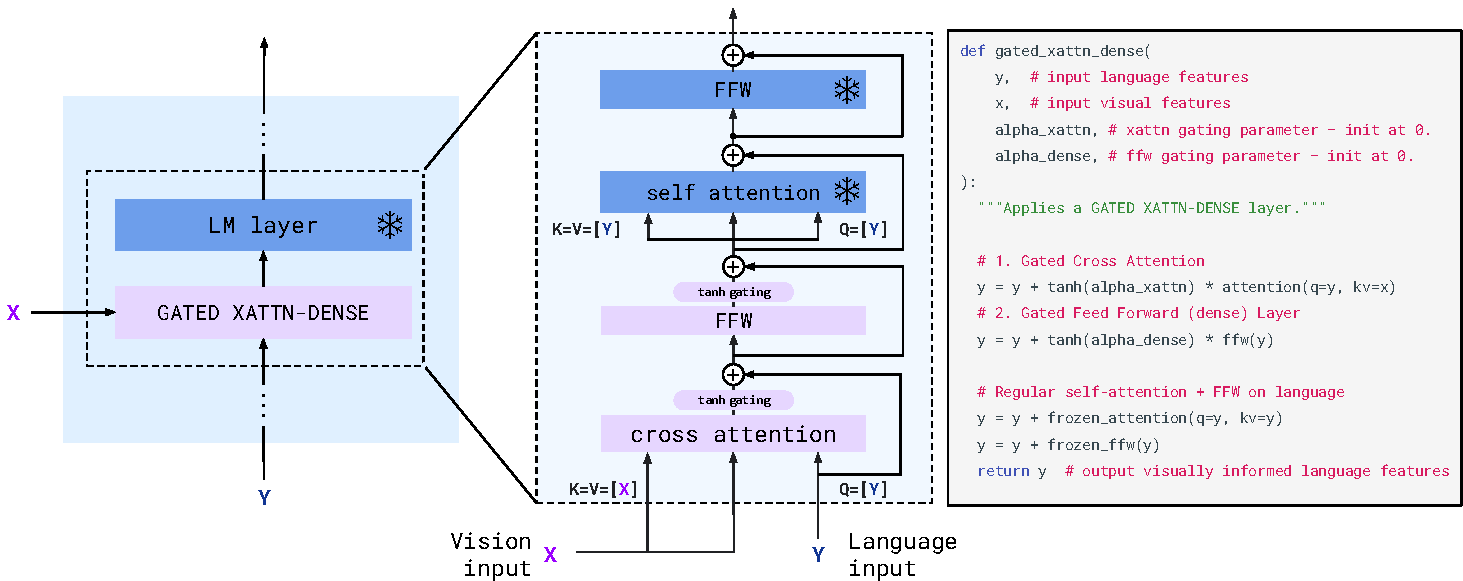
\includegraphics[width=\linewidth]{figures/fig4_xattn_dense.pdf}
\centering
\caption{\capfontsize{} \textbf{\textsc{gated xattn-dense} layers.} 为了使 LM 以视觉输入为条件,我们在现有的预训练和冻结 LM 层之间插入了新的交叉注意层。这些层中的键和值来自视觉特征,而查询则来自语言输入。
这些层之后是密集的前馈层。
这些层是\emph{gated}的,因此 LM 在初始化时保持不变,以提高稳定性和性能。}
\label{fig:xattn_dense}
\end{figure}

\textbf{在冻结的预训练 LM 中插入新的\textsc{门控交叉注意密集gated cross attention dense}层}。
我们冻结了预训练的 LM 块,并在(从头开始训练的)原始层之间插入\textit{gated cross attention dense})块(Figure~\ref{fig:xattn_dense})。
为了确保在初始化时,条件化模型能产生与原始语言模型相同的结果,我们使用了一种 $\tanh$ 门控机制。
这将新添加层的输出乘以 $\tanh(\alpha)$,然后再将其添加到来自残差连接的输入表示中,其中 $\alpha$ 是一个特定于层的可学习标量,初始化为 $0$ ~\cite{bachlechner2021rezero})。
因此,在初始化时,模型输出与预训练的 LM 相匹配,从而提高了训练的稳定性和最终性能。
在消融研究(Section~\ref{sec:ablations})中,我们将所提出的\textsc{gated xattn-dense}层与最近的替代方法进行了比较~\citep{desai2021virtex,luo2022vc},并探索了插入这些附加层的频率对效率和表现力之间权衡的影响。
详见附录~\maintoappref{app:xattn_dense}。


\textbf{Varying model sizes.}
我们在 1.4B、7B 和 70B 参数的Chinchilla模型~\citep{chinchilla}基础上,对三种模型大小进行了实验;分别称它们为 \base{})、 \medium{})和 \largemfull{}。
为简洁起见,我们在本文中将最后一个称为\largem{}。
在增加冷冻 LM 模块和可训练视觉文本\textsc{gated xattn-dense} 模块的参数数量的同时,我们在不同的模型中保持了固定大小的冷冻视觉编码器和可训练感知器重采样器(相对于完整模型大小较小)。
更多详情请参见附录~\maintoappref{sec:models_details}。



\subsection{Multi-visual input support: per-image/video attention masking}
\label{sec:multi_im_att}

等式~\eqref{eq:modeling}中引入的图像因果建模是通过屏蔽完整的文本-图像交叉注意力矩阵来实现的、
限制模型在每个文本标记处看到的视觉标记。
在给定的文本标记处,模型会关注交错序列中出现在它之前的图像的视觉标记,而不是之前的所有图像(在附录~\maintoappref{app:multi-visual-details}中进行了形式化和说明)。
虽然该模型每次只\textit{直接}关注一幅图像,但通过 LM 中的自我关注,对之前所有图像的依赖性仍然存在。
这种单张图像交叉关注方案的重要意义在于,无论在训练过程中使用了多少张图像,模型都能无缝泛化到任意数量的视觉输入。
特别是,我们在交错数据集上进行训练时,每个序列最多只能使用 5 张图片,但在评估过程中,我们的模型却能从多达 32 对(或 `shots'')图片/视频和相应文本的序列中获益。
我们将在第~\ref{sec:ablations}节中证明,这种方案比让模型直接交叉关注之前的所有图像更为有效。



\subsection{Training on a mixture of vision and language datasets}
\label{sec:datasets}\label{sec:training}


我们在三种数据集的混合数据集上训练 \method{} 模型,所有数据集均来自网络:来自网页的交错图像和文本数据集、图像-文本对和视频-文本对。


\textbf{M3W: Interleaved image and text dataset.}
\label{sec:interleaved_datasets}
Flamingo 模型的少样本能力依赖于对交错文本和图像数据的训练。
为此,我们收集了 \emph{MultiModal MassiveWeb} (\mmmw) 数据集。
我们从大约 4,300 万个网页的 HTML 中提取文本和图像,根据文本和图像元素在文档对象模型(DOM)中的相对位置,确定图像相对于文本的位置。
然后,在页面上图像的位置插入纯文本中的\texttt{<image>}标记,并在任何图像之前和文档末尾插入一个特殊的\texttt{<EOC>}(\textit{end chunk})标记,从而构建一个示例。\textit{end of chunk})标记(添加到词汇表中并被学习)。
我们从每篇文档中随机抽取 $L=256$ 标记的子序列,并取样序列中包含的最多 $N=5$ 图片。
为了节省计算量,后面的图像将被舍弃。
更多详情见附录~\maintoappref{app:datasets}。

\textbf{图像/视频和文本的配对}。
对于图像和文本配对,我们首先利用了 ALIGN~\citep{align} 数据集,该数据集由 18 亿张与 alt-text 配对的图像组成。
作为对该数据集的补充,我们还收集了自己的图像和文本配对数据集,目标是质量更好、描述更长的图像和文本:  \shortimagetextpairs{} (\imagetextpairs)由 3.12 亿张图片和文本对组成。
我们还收集了一个类似的数据集,但使用的是视频而不是静态图像: \shortvideotextpairs(\videotextpairs)由 2,700 万个短视频(平均约 22 秒)和句子描述组成。
我们通过在每个训练标题前添加\texttt{<image>}和附加\texttt{<EOC>},使配对数据集的语法与M3W的语法保持一致(详见附录~\maintoappref{app:vtp_and_itp})。

\textbf{Multi-objective training and optimisation strategy.}
在视觉输入的情况下,我们通过最小化每个数据集文本预期负对数似然的加权和来训练模型:
\begin{equation}
    \sum_{m=1}^{M} \lambda_m \cdot \mathbb{E}_{(x, y)\sim \mathcal{D}_m} \left[ -\sum_{\ell=1}^L \log p(y_\ell | y_{< \ell}, x_{\leq \ell})\right],
\end{equation}
其中,$mathcal{D}_m$ 和 $\lambda_m$ 分别是 $m$ 数据集及其权重。
调整每个数据集的权重 $\lambda_m$ 是提高性能的关键。
我们在所有数据集上累积梯度,发现这种方法优于 "轮循 "``round-robin''方法~\citep{cho2021unifying}。
我们在附录中提供了进一步的训练细节和消融~\maintoappref{app:large_scale_training}。

\subsection{Task adaptation with few-shot in-context learning}
\label{sec:adapt-vlm}

训练好Flamingo后,我们用它来完成一项视觉任务,即对多模态交错提示进行调节。%
我们使用文本学习\textbf{in-context learning})来评估我们的模型快速适应新任务的能力,类似于 GPT-3~\citep{gpt3},方法是以 $(image, text)$ or $(video, text)$ 的形式交错支持示例对,然后是查询视觉输入,从而建立一个提示(详情见附录~\maintoappref{app:in_context_eval_details})。
我们使用波束搜索进行解码,并使用我们模型的对数似然对每个可能的答案进行评分,从而执行\textbf{open-ended}评估。
我们探索了 \textbf{zero-shot generalization},方法是用任务中的两个纯文本示例(没有相应的图像)来提示模型。
评估超参数和其他细节见附录~\maintoappref{app:fewshot-eval-hyper}。



\section{Experiments}
\label{sec:experiments}
我们的目标是开发能够快速适应各种挑战性任务的模型。
为此,我们考虑了 16 种流行的多模态图像/视频和语言基准。
为了在项目过程中验证模型设计决策,其中 5 个基准被用作我们开发(\dev{})集的一部分: COCO、OKVQA、VQAv2、MSVDQA 和 VATEX。
由于模型选择的原因,对 \dev{} 基准的性能估计可能存在偏差。
我们注意到,先前利用类似基准验证和消减设计决策的工作也存在这种情况。
为此,我们额外报告了 11 个基准的性能、
这些基准包括字幕、视频问题解答,以及一些不太常见的功能,如视觉对话和多选问题解答任务。
附录~\maintoappref{sec:eval_benchmarks}中描述了评估基准。
在所有基准中,我们保持所有评估超参数固定不变。
根据任务的不同,我们使用了四种少量提示模板,更多详情请参见 
Appendix~\maintoappref{app:fewshot-eval-hyper} 中详细介绍。
我们强调,\emph{我们并没有在这 11 个基准上验证任何设计决策},而只是用它们来估计我们模型的无偏少量unbiased few-shot学习性能。


具体来说,要估算一个模型的few-shot学习性能,需要用一组 \emph{support} 样本对其进行提示,然后在一组 \emph{query} 样本上对其进行评估。
对于用于验证设计决策和超参数以及报告最终性能的 \dev{} 基准,我们使用了四个子集:
\metadevsupportshort{}、\metadevqueryshort{}、\metatestsupportshort{}和\metatestqueryshort{}。
对于其他基准,我们只需要后两个。
我们将在附录~\maintoappref{sec:eval_benchmarks}中报告如何形成这些子集。

我们将在第~\ref{sec:fewshot_openended}节中报告~\method{}模型在few-shot学习上的结果。
第~\ref{sec:ft_results}节给出了微调结果。
消融研究见第~\ref{sec:ablations}节。
附录~\maintoappref{app:more_performance}提供了更多结果,包括\method{}在ImageNet和Kinetics700分类任务中的表现,以及我们的对比模型的表现。
附录~\maintoappref{app:qual_res}包含了更多定性结果。





\subsection{Few-shot learning on vision-language tasks}
\label{sec:fewshot_openended}


\begin{table}[t]
\resizebox{\textwidth}{!}{%
\begin{tabular}{ccccccccccccccccccc}
\toprule
Method                                                                        & FT                & Shot                                                                            & \rotatebox[origin=c]{90}{OKVQA \textbf{(I)}}                                                                              & \rotatebox[origin=c]{90}{VQAv2 \textbf{(I)}}                                                                                      & \rotatebox[origin=c]{90}{COCO \textbf{(I)}}                                                                                      & \rotatebox[origin=c]{90}{MSVDQA \textbf{(V)}}                                                                                & \multicolumn{1}{c}{\rotatebox[origin=c]{90}{VATEX \textbf{(V)}}}                                                             & \rotatebox[origin=c]{90}{VizWiz \textbf{(I)}}                                                                                 & \rotatebox[origin=c]{90}{Flick30K \textbf{(I)}}                                                                                 & \rotatebox[origin=c]{90}{MSRVTTQA \textbf{(V)}}                                                                               & \rotatebox[origin=c]{90}{iVQA \textbf{(V)}}                                                                                 & \multicolumn{1}{c}{\rotatebox[origin=c]{90}{YouCook2 \textbf{(V)}}}                                                       & \rotatebox[origin=c]{90}{STAR \textbf{(V)}}                                                                                & \rotatebox[origin=c]{90}{VisDial \textbf{(I)}}                                                                                     & \rotatebox[origin=c]{90}{TextVQA \textbf{(I)}}                                                                              & \rotatebox[origin=c]{90}{NextQA \textbf{(I)}}                                                                                & \rotatebox[origin=c]{90}{\phantom{a}HatefulMemes \textbf{(I)}\phantom{a}}                                                                           & \rotatebox[origin=c]{90}{RareAct \textbf{(V)}}                                             \\ \hline
\begin{tabular}[c]{@{}c@{}}Zero/Few \\ shot SOTA\end{tabular}                 & \ding{55}         & \begin{tabular}[c]{@{}c@{}}\phantom{0}\\ \phantom{0}\\ (X)\end{tabular}         & \begin{tabular}[c]{@{}c@{}}\small{[\citenum{gui2021kat}]}\\ 43.3 \\ (16)\end{tabular}                         & \begin{tabular}[c]{@{}c@{}}\small{[\citenum{tsimpoukelli2021multimodal}]}\\ 38.2\\ (4)\end{tabular}                  & \begin{tabular}[c]{@{}c@{}}\small{[\citenum{wang2021simvlm}]}\\ 32.2\\ (0)\end{tabular}                             & \begin{tabular}[c]{@{}c@{}}\small{[\citenum{li2022blip}]}\\ 35.2\\ (0)\end{tabular}                             & -                                                                                                                & -                                                                                                                & -                                                                                                                  & \begin{tabular}[c]{@{}c@{}}\small{[\citenum{li2022blip}]}\\ 19.2\\ (0)\end{tabular}                              & \begin{tabular}[c]{@{}c@{}}\small{[\citenum{yang2021just}]}\\ 12.2\\ (0)\end{tabular}                          & -                                                                                                             & \begin{tabular}[c]{@{}c@{}}\small{[\citenum{zellers2022merlot}]}\\ 39.4\\ (0)\end{tabular}                    & \begin{tabular}[c]{@{}c@{}}\small{[\citenum{murahari2020large}]}\\ 11.6\\ (0)\end{tabular}                            & -                                                                                                              & -                                                                                                               & \begin{tabular}[c]{@{}c@{}}\small{[\citenum{clip}]}\\ 66.1\\ (0)\end{tabular}                                    & \begin{tabular}[c]{@{}c@{}}\small{[\citenum{clip}]}\\ 40.7\\ (0)\end{tabular} \\ \hline
\multirow{3}{*}{\base{}}                                                      & \ding{55}         & 0                                                                               & 41.2                                                                                                          & 49.2                                                                                                                 & 73.0                                                                                                                & 27.5                                                                                                            & 40.1                                                                                                             & 28.9                                                                                                             & 60.6                                                                                                               & 11.0                                                                                                             & 32.7                                                                                                           & 55.8                                                                                                          & 39.6                                                                                                          & 46.1                                                                                                                  & 30.1                                                                                                           & 21.3                                                                                                            & 53.7                                                                                                             & 58.4                                                                          \\
                                                                              & \ding{55}         & 4                                                                               & 43.3                                                                                                          & 53.2                                                                                                                 & 85.0                                                                                                                & 33.0                                                                                                            & 50.0                                                                                                             & 34.0                                                                                                             & 72.0                                                                                                               & 14.9                                                                                                             & 35.7                                                                                                           & 64.6                                                                                                          & 41.3                                                                                                          & 47.3                                                                                                                  & 32.7                                                                                                           & 22.4                                                                                                            & 53.6                                                                                                             & -                                                                             \\
                                                                              & \ding{55}         & 32                                                                              & 45.9                                                                                                          & 57.1                                                                                                                 & 99.0                                                                                                                & 42.6                                                                                                            & 59.2                                                                                                             & 45.5                                                                                                             & 71.2                                                                                                               & 25.6                                                                                                             & 37.7                                                                                                           & 76.7                                                                                                          & 41.6                                                                                                          & 47.3                                                                                                                   & 30.6                                                                                                           & 26.1                                                                                                            & 56.3                                                                                                             & -                                                                             \\ \hline
\multirow{3}{*}{\medium{}}                                                    & \ding{55}         & 0                                                                               & 44.7                                                                                                          & 51.8                                                                                                                 & 79.4                                                                                                                & 30.2                                                                                                            & 39.5                                                                                                             & 28.8                                                                                                             & 61.5                                                                                                               & 13.7                                                                                                             & 35.2                                                                                                           & 55.0                                                                                                          & 41.8                                                                                                          & 48.0                                                                                                                  & 31.8                                                                                                           & 23.0                                                                                                            & 57.0                                                                                                             & 57.9                                                                          \\
                                                                              & \ding{55}         & 4                                                                               & 49.3                                                                                                          & 56.3                                                                                                                 & 93.1                                                                                                                & 36.2                                                                                                            & 51.7                                                                                                             & 34.9                                                                                                             & 72.6                                                                                                               & 18.2                                                                                                             & 37.7                                                                                                           & 70.8                                                                                                          & {\ul \textbf{42.8}}                                                                                                          & 50.4                                                                                                                  & 33.6                                                                                                           & 24.7                                                                                                            & 62.7                                                                                                             & -                                                                             \\
                                                                              & \ding{55}         & 32                                                                              & 51.0                                                                                                          & 60.4                                                                                                                 & 106.3                                                                                                               & 47.2                                                                                                            & 57.4                                                                                                             & 44.0                                                                                                             & 72.8                                                                                                               & 29.4                                                                                                             & 40.7                                                                                                           & 77.3                                                                                                          & 41.2                                                                                                          & 50.4                                                                                                                  & 32.6                                                                                                           & 28.4                                                                                                            & 63.5                                                                                                             & -                                                                             \\ \hline
\multirow{4}{*}{\largem{}}                                                    & \ding{55}         & 0                                                                               & 50.6                                                                                                          & 56.3                                                                                                                 & 84.3                                                                                                                & 35.6                                                                                                            & 46.7                                                                                                             & 31.6                                                                                                             & 67.2                                                                                                               & 17.4                                                                                                             & 40.7                                                                                                           & 60.1                                                                                                          & 39.7                                                                                                          & 52.0                                                                                                                  & 35.0                                                                                                           & 26.7                                                                                                            & 46.4                                                                                                             & {\ul \textbf{60.8}}                                                           \\
                                                                              & \ding{55}         & 4                                                                               & 57.4                                                                                                          & 63.1                                                                                                                 & 103.2                                                                                                               & 41.7                                                                                                            & 56.0                                                                                                             & 39.6                                                                                                             & 75.1                                                                                                               & 23.9                                                                                                             & 44.1                                                                                                           & 74.5                                                                                                          & 42.4                                                                                                          & \textbf{55.6}                                                                                                                  & 36.5                                                                                                           & 30.8                                                                                                            & 68.6                                                                                                             & -                                                                             \\
                                                                              & \ding{55}         & 32                                                                              & {\ul \textbf{57.8}}                                                                                           & \textbf{67.6}                                                                                                        & \textbf{113.8}                                                                                                      & {\ul \textbf{52.3}}                                                                                             & \textbf{65.1}                                                                                                    & \textbf{49.8}                                                                                                    & {\ul \textbf{75.4}}                                                                                                               & \textbf{31.0}                                                                                                    & {\ul \textbf{45.3}}                                                                                            & \textbf{86.8}                                                                                                 & 42.2                                                                                                          & \textbf{55.6}                                                                                                                   & \textbf{37.9}                                                                                                  & {\ul \textbf{33.5}}                                                                                             & \textbf{70.0}                                                                                                    & -                                                                             \\ \hline
\begin{tabular}[c]{@{}c@{}}\vlpft{Pretrained}\\  \vlpft{FT SOTA}\end{tabular} & \vlpft{\ding{52}} & \begin{tabular}[c]{@{}c@{}}\phantom{0}\\ \phantom{0}\\ \vlpft{(X)}\end{tabular} & \begin{tabular}[c]{@{}c@{}}\vlpft{54.4}\\ \vlpft{\small{[\citenum{gui2021kat}]}}\\ \vlpft{(10K)}\end{tabular} & \begin{tabular}[c]{@{}c@{}}\vlpft{80.2}\\ \vlpft{\small{[\citenum{yuan2021florence}]}}\\ \vlpft{(444K)}\end{tabular} & \begin{tabular}[c]{@{}c@{}}\vlpft{143.3}\\ \vlpft{\small{[\citenum{wang2021simvlm}]}}\\ \vlpft{(500K)}\end{tabular} & \begin{tabular}[c]{@{}c@{}}\vlpft{47.9}\\ \vlpft{\small{[\citenum{fu2021violet}]}}\\ \vlpft{(27K)}\end{tabular} & \begin{tabular}[c]{@{}c@{}}\vlpft{76.3}\\ \vlpft{\small{[\citenum{zhu2019vatex}]}}\\ \vlpft{(500K)}\end{tabular} & \begin{tabular}[c]{@{}c@{}}\vlpft{57.2}\\ \vlpft{\small{[\citenum{liu2021vizwiz}]}}\\ \vlpft{(20K)}\end{tabular} & \begin{tabular}[c]{@{}c@{}}\vlpft{67.4}\\ \vlpft{\small{[\citenum{zhou2020unified}]}}\\ \vlpft{(30K)}\end{tabular} & \begin{tabular}[c]{@{}c@{}}\vlpft{46.8}\\ \vlpft{\small{[\citenum{wang2022allinone}]}}\\ \vlpft{(130K)}\end{tabular} & \begin{tabular}[c]{@{}c@{}}\vlpft{35.4}\\ \vlpft{\small{[\citenum{yang2021just}]}}\\ \vlpft{(6K)}\end{tabular} & \begin{tabular}[c]{@{}c@{}}\vlpft{138.7}\\ \vlpft{\small{[\citenum{xu2021vlm}]}}\\ \vlpft{(10K)}\end{tabular} & \begin{tabular}[c]{@{}c@{}}\vlpft{36.7}\\ \vlpft{\small{[\citenum{wu2021star}]}}\\ \vlpft{(46K)}\end{tabular} & \begin{tabular}[c]{@{}c@{}}\vlpft{75.2}\\ \vlpft{\small{[\citenum{murahari2020large}]}}\\ \vlpft{(123K)}\end{tabular} & \begin{tabular}[c]{@{}c@{}}\vlpft{54.7}\\ \small{\vlpft{[\citenum{yang2021tap}}]}\\ \vlpft{(20K)}\end{tabular} & \begin{tabular}[c]{@{}c@{}}\vlpft{25.2}\\ \vlpft{\small{[\citenum{xiao2021next}]}}\\ \vlpft{(38K)}\end{tabular} & \begin{tabular}[c]{@{}c@{}}\vlpft{79.1}\\ \vlpft{\small{[\citenum{lippe2020multimodal}]}}\\ \vlpft{(9K)}\end{tabular} & -                                                                             \\ \bottomrule
\end{tabular}
}

\vspace{0.5em}

\caption{
\capfontsize{}
\label{tab:fewshot_all_tasks} \textbf{Comparison to the state of the art.} A \emph{single} Flamingo model reaches the state of the art on a wide array of image \textbf{(I)} and video \textbf{(V)} understanding tasks with few-shot learning, significantly outperforming previous best zero- and few-shot methods with as few as four examples.
More importantly, using only $32$ examples and without adapting any model weights, \method{} {\em outperforms} the current best methods -- fine-tuned on thousands of annotated examples -- on seven tasks.
Best few-shot numbers are in \textbf{bold}, best numbers overall are {\ul underlined}. 
}
\vspace{-0.5cm}
\end{table}



\textbf{Few-shot results.}
结果见表~\ref{tab:lewshot_all_tasks}。
\largem{}在所考虑的 16 项基准测试中,\largem{} 远远优于之前的\emph{all}zero-shot或few-shot测试方法。
每个任务只需四个示例就能实现这一目标,这证明了视觉模型适应新任务的实用性和高效性。
更重要的是,\largem{}通常可以在多达数十万个注释示例的基础上进行微调,从而与最先进的方法相媲美。
在六项任务中,\largem{}甚至优于经过微调的 SotA,尽管它只使用了\emph{一组}模型权重和 32 个特定任务示例。
最后,尽管我们只使用了 \dev{} 基准来进行设计决策,但我们的结果还是很好地推广到了其他基准,这也证实了我们方法的通用性。


\textbf{Scaling with respect to parameters and shots.}
As shown in Figure~\ref{fig:results}, the larger the model, the better the few-shot performance, similar to GPT-3~\citep{gpt3}.
The performance also improves with the number of shots.
We further find that the largest model better exploits larger numbers of shots.
Interestingly, even though our \method{} models were trained with sequences limited to only 5 images on \mmmw{}, they are still able to benefit from up to 32 images or videos during inference.
This demonstrates the flexibility of the \method{} architecture for processing a variable number of videos or images.

\textbf{Scaling with respect to parameters and shots.与参数和样本有关的缩放}。
如图~\ref{fig:results}所示,模型越大,少镜头性能越好,这与 GPT-3~\citep{gpt3} 类似。
性能也随着拍摄次数的增加而提高。
我们进一步发现,最大的模型能更好地利用更多的镜头。
有趣的是,尽管我们的 \method{}模型在 \mmmw{}上的训练序列仅限于 5 幅图像,但它们在推理过程中仍能从多达 32 幅图像或视频中获益。
这证明了 \method{} 架构在处理不同数量的视频或图像时的灵活性。


\subsection{Fine-tuning \largem{} as a pretrained vision-language model}
\label{sec:ft_results}

虽然这并不是我们工作的重点,但我们验证了当给定更多数据时,\method{}模型可以通过微调权重来适应任务。
在表~\ref{tab:ft-sota-table-compressed}中,我们探索了在注释预算不受限制的情况下,针对给定任务微调我们最大的模型\largem{})。
简而言之,我们通过在较短的时间内以较小的学习率对模型进行微调,另外解冻视觉骨干网以适应更高的输入分辨率(详情见附录~in Appendix~\maintoappref{app:finetuning})。
我们发现,与之前介绍的在上下文中进行少量学习的结果相比,我们可以改进结果,在另外五项任务中创造了新的技术水平: VQAv2、VATEX、VizWiz、MSRVTTQA 和 HatefulMemes。

\newcommand{\uln}[1]{\underline{#1}}
\newcommand{\bo}[1]{\bf{\underline{#1}}}
\newcommand{\ofa}{\footnotesize{[\citenum{wang2022unifying}]}}
\newcommand{\simvlm}{\footnotesize{[\citenum{wang2021simvlm}]}}
\newcommand{\florence}{\footnotesize{[\citenum{yuan2021florence}]}}
\newcommand{\alice}{\footnotesize{[\citenum{yan2021achieving}]}}
\newcommand{\vatex}{\footnotesize{[\citenum{zhu2019vatex}]}}
\newcommand{\vizwiz}{\footnotesize{[\citenum{liu2021vizwiz}]}}
\newcommand{\allinon}{\footnotesize{[\citenum{wang2022allinone}]}}
\newcommand{\visdial}{\footnotesize{[\citenum{murahari2020large}]}}
\newcommand{\vdbert}{\footnotesize{[\citenum{wang2020vdbert}]}}
\newcommand{\youcook}{\footnotesize{[\citenum{xu2021vlm}]}}
\newcommand{\tap}{\footnotesize{[\citenum{yang2021tap}]}}
\newcommand{\teammia}{\footnotesize{[\citenum{qiao2021winner}]}}
\newcommand{\flava}{\footnotesize{[\citenum{singh2021flava}]}}
\newcommand{\hateful}{\footnotesize{[\citenum{lippe2020multimodal}]}}
\newcommand{\zhu}{\footnotesize{[\citenum{zhu2020enhance}]}}
\newcommand{\sota}{SotA}

\begin{table*}[t]
\resizebox{\textwidth}{!}{%
\begin{tabular}{rccccccccccccc}
\hline
Method            & \multicolumn{2}{c|}{VQAV2} & \multicolumn{1}{c|}{COCO} & \multicolumn{1}{c|}{VATEX} & \multicolumn{2}{c|}{VizWiz} & \multicolumn{1}{c|}{MSRVTTQA} & \multicolumn{2}{c|}{VisDial} & \multicolumn{1}{c|}{YouCook2} & \multicolumn{2}{c|}{TextVQA} & \multicolumn1{c}{HatefulMemes} \\
                  & test-dev       & \multicolumn{1}{c|}{test-std}       & \multicolumn{1}{c|}{test}                           & \multicolumn{1}{c|}{test}                            & test-dev        & \multicolumn{1}{c|}{test-std}       & \multicolumn{1}{c|}{test}                               & \multicolumn{1}{c|}{valid}                              & \multicolumn{1}{c|}{test-std}                              & \multicolumn{1}{c|}{valid}        & \multicolumn{1}{c|}{valid}        & \multicolumn{1}{c|}{test-std}         & \multicolumn{1}{c}{test seen}                                   \\ \hline
\flamingoemoji{} 32 shots&67.6     &  -      & 113.8    & 65.1    & 49.8     & -       &   31.0  & 56.8  &  -  & 86.8    & 36.0     &  -  & 70.0   \\
\flamingoemoji{} Fine-tuned &\bo{82.0}&\bo{82.1}&  138.1   &\bo{84.2}&\bo{65.7}&\bf{65.4}&\bf{47.4}& 61.8 & 59.7 &  118.6  &\bf{57.1}&54.1      &\bo{86.6}\\
\hline
                                     &   81.3$^\dagger$ & 81.3$^\dagger$    &\bf{149.6}$^\dagger$&  81.4$^\dagger$  &  57.2$^\dagger$    &   60.6$^\dagger$  &    46.8   & \bf{75.2}   &   \bf{75.4}$^\dagger$    &   \bf{138.7}   &   54.7   &   \bf{73.7}    & 84.6$^\dagger$\\
\multirow{-2}{*}{\sota}             &\alice   &\alice   &   \ofa   & \vatex  &     \vizwiz     & \vizwiz&   \allinon  &    \visdial  & \vdbert &    \youcook &   \tap   &  \teammia     & \zhu \\
\hline
\end{tabular}%
}
\caption{
\capfontsize{} \label{tab:ft-sota-table-compressed} \textbf{Comparison to SotA when fine-tuning \largem{}.}
We fine-tune~\largem{} on all nine tasks where \largem{} does not achieve SotA with few-shot learning.
\largem{} sets a new SotA on five of them, outperfoming methods (marked with $\dagger$) that use tricks such as model ensembling or domain-specific metric optimisation (e.g., CIDEr optimisation).}
\end{table*}


\subsection{Ablation studies}
\label{sec:ablations}


\begin{table}[t]
\resizebox{\textwidth}{!}{%
\begin{tabular}{@{}rlll|cc|ccccc|cc@{}}
\toprule
&Ablated  & \base{} & Changed & \small{Param.}  &            \small{Step}     & COCO & OKVQA & VQAv2  & MSVDQA & VATEX & Overall \\
&setting & original value & value  & \small{count $\downarrow$}  &   \small{time $\downarrow$}               & CIDEr$\uparrow$  & top1$\uparrow$ & top1$\uparrow$     & top1$\uparrow$   & CIDEr$\uparrow$  &   score$\uparrow$   \\ \midrule
&\multicolumn{3}{c|}{\textbf{\base{} model}}    & 3.2B & 1.74s &   86.5  &   42.1    &  55.8        &     36.3     &  53.4     &  \textbf{70.7}     \\ \midrule
\multirow{4}{*}{\textbf{(i)}}&\multirow{4}{*}{Training data} & \multirow{4}{*}{All data} & w/o Video-Text pairs &  3.2B & 1.42s &  84.2 &   43.0  &  53.9  &  34.5  &  46.0  & 67.3    \\
& &  & w/o Image-Text pairs    &  3.2B &  0.95s &  66.3 &   39.2  &  51.6    &  32.0  &  41.6  &  60.9   \\
& &  & Image-Text pairs$\rightarrow$ LAION    &  3.2B &  1.74s &  79.5 &   41.4  &  53.5    &  33.9  &  47.6  &  66.4   \\
& &  & w/o M3W & 3.2B &  1.02s                  &  54.1  &  36.5  &  52.7&  31.4  &  23.5  &  53.4  \\  \midrule
\textbf{(ii)}& Optimisation & Accumulation  & Round Robin & 3.2B & 1.68s &   76.1 & 39.8   &  52.1   &   33.2    & 40.8  &  62.9 \\  \midrule
\textbf{(iii)} & Tanh gating & \ding{51}  &  \ding{55} & 3.2B & 1.74s &  78.4 & 40.5   &  52.9      &    35.9    &  47.5     &     66.5    \\  \midrule
\multirow{2}{*}{\textbf{(iv)}}& Cross-attention  & \multirow{2}{*}{\shortstack[c]{\textsc{gated}\\\textsc{xattn-dense}}} & \small{\textsc{Vanilla xattn}}  & 2.4B & 1.16s &   80.6 & 41.5    &   53.4     &    32.9    &   50.7    &   66.9    \\ 	
&architecture  & & \small{\textsc{Grafting}}   & 3.3B & 1.74s &   79.2  & 36.1   &  50.8     &   32.2    &    47.8   &   63.1      \\ \midrule
\multirow{3}{*}{\textbf{(v)}}&\multirow{3}{*}{\shortstack[l]{Cross-attention\\ frequency}} & \multirow{3}{*}{Every}  & Single in middle & 2.0B & 0.87s &  71.5  & 38.1 &   50.2       &    29.1    &  42.3  &   59.8    \\  					
& & & Every 4th &  2.3B & 1.02s  &   82.3  & 42.7    &    55.1       &    34.6    &   50.8    &   68.8    \\ 						
& & & Every 2nd &  2.6B & 1.24s  &   83.7  & 41.0    &   55.8      &  34.5      &   49.7    &   	    68.2   \\  \midrule 		
\multirow{2}{*}{\textbf{(vi)}}& \multirow{2}{*}{Resampler}  & \multirow{2}{*}{Perceiver}  & MLP &  3.2B & 1.85s &   78.6 &  42.2     &   54.7     &    35.2    &  44.7     &  66.6      \\				
& & &  Transformer &  3.2B & 1.81s  &  83.2 &  41.7     &   55.6       &   31.5     &  48.3     &   66.7     \\  \midrule
\multirow{2}{*}{\textbf{(vii)}}&\multirow{2}{*}{Vision encoder} & \multirow{2}{*}{NFNet-F6}  &  CLIP ViT-L/14 & 3.1B & 1.58s   &  76.5 & 41.6    &   53.4      &   33.2     &   44.5    &    64.9    \\  	
& & &  NFNet-F0 & 2.9B & 1.45s  &    73.8 & 40.5     &  52.8       &    31.1    &  42.9     &    62.7  \\ \midrule
\multirow{2}{*}{\textbf{(viii)}}& \multirow{2}{*}{Freezing LM} & \multirow{2}{*}{\ding{51}}  & \ding{55} (random init)   &  3.2B & 2.42s &  74.8 & 31.5   &  45.6    &  26.9   &  50.1 &  57.8  \\
& &  & \ding{55}  (pretrained)   &  3.2B & 2.42s &   81.2  & 33.7   &  47.4 &   31.0    &    53.9  &   62.7      \\  \midrule
\end{tabular}%
}
\caption{\capfontsize{} \textbf{Ablation studies.} 
Each row should be compared to the baseline~\method{} run (top row).
Step time measures the time spent to perform gradient updates on all training datasets.
}
\vspace{-0.4cm}
\label{tab:ablation-table-no-classif}
\end{table}



In Table~\ref{tab:ablation-table-no-classif}, we report our ablation results using \base{}~on the \metadevsubsets~of the five \dev{} benchmarks with 4 shots.
Note that we use smaller batch sizes and a shorter training schedule compared to the final models.
The \textbf{Overall score} is obtained by dividing each benchmark score by its state-of-the-art (SotA) performance from Table~\ref{tab:fewshot_all_tasks} and averaging the results.
More details and results are given in Appendix~\maintoappref{app:all_ablation_studies} and Table~\ref{tab:ablation-table-appendix}.

\noindent
\textbf{Importance of the training data mixture.}
As shown in row \textbf{(i)}, getting the right training data plays a crucial role.
In fact, removing the interleaved image-text dataset \mmmw{} leads to a \emph{decrease of more than $17\%$} in performance while removing the conventional paired image-text pairs also decreases performance (by $9.8\%$), demonstrating the need for different types of datasets.
Moreover, removing our paired video-text dataset negatively affects performance on all video tasks.
We ablate replacing our image-text pairs (ITP) by the publicly available LAION-400M dataset~\cite{schuhmann2021laion}, which leads to a slight degradation in performance.
We show in row \textbf{(ii)} the importance of our gradient accumulation strategy compared to using round-robin updates~\citep{cho2021unifying}.

 \textbf{Importance of the training data mixture.}
 如\textbf{(i)}行所示,获取正确的训练数据起着至关重要的作用。 事实上,去除交错的图像-文本数据集\mmmw{}会导致\emph{下降超过$17\%$},而去除传统的配对图像-文本数据对也会降低性能(by $9.8\%$),这表明需要不同类型的数据集。
 此外,去除我们的配对视频-文本数据集会对所有视频任务的性能产生负面影响。 
 我们进行了替换公开可用的LAION-400M数据集~\cite{schuhmann2021laion}来代替我们的图像-文本配对(ITP)的实验,结果发现性能略有下降。 我们在\textbf{(ii)}行展示了我们的梯度累积策略与使用轮询更新~\citep{cho2021unifying}的重要性。

\noindent   
\textbf{Visual conditioning of the frozen LM.}
We ablate the use of the 0-initialized tanh gating when merging the cross-attention output to the frozen LM output in row \textbf{(iii)}.
Without it, we see a drop of $4.2\%$ in our overall score.
Moreover, we have noticed that disabling the 0-initialized tanh gating leads to training instabilities.
Next, we ablate different conditioning architectures in row \textbf{(iv)}.
\textsc{vanilla xattn}, refers to the vanilla cross-attention from the original Transformer decoder~\citep{vaswani2017attention}.
In the \textsc{grafting} approach from~\cite{luo2022vc}, the frozen LM is used as is with no additional layers inserted, and a stack of interleaved self-attention and cross-attention layers that take the frozen LM output are learnt from scratch.
Overall, we show that our \textsc{gated xattn-dense} conditioning approach works best.

\noindent
\textbf{Compute/Memory vs. performance trade-offs.}
In row \textbf{(v)}, we ablate the frequency at which we add new \textsc{gated xattn-dense} blocks.
Although adding them at every layer is better, it significantly increases the number of trainable parameters and time complexity of the model.
Notably, inserting them every fourth block accelerates training by $66\%$ while only decreasing the overall score by $1.9\%$.
In light of this trade-off, we maximize the number of added layers under hardware constraints and add a \textsc{gated xattn-dense} every fourth layer for \medium{} and every seventh for \largemfull{}.
We further compare in row \textbf{(vi)} the Perceiver Resampler to a MLP and a vanilla Transformer given a parameter budget.
Both underperform the Perceiver Resampler while also being slower.


\noindent
\textbf{Vision encoder.}
In row \textbf{(vii)}, we compare our NFNet-F6 vision encoder pretrained with contrastive learning \newreferencetoappendix{(details in Appendix~\maintoappref{app:contrastive_details})} to the publicly available CLIP ViT-L/14~\citep{clip} model trained at 224 resolution.
Our NFNet-F6 has a $+5.8\%$ advantage over the CLIP ViT-L/14 and $+8.0\%$ over a smaller NFNet-F0 encoder, which highlights the importance of using a strong vision backbone.

\noindent
\textbf{Freezing LM components prevents catastrophic forgetting.} %
我们在第\textbf{(viii)}行中验证了在训练时冻结 LM 层的重要性。
如果从头开始训练,我们观察到性能会大幅下降 $-12.9\%$。
有趣的是,对我们预训练的 LM 进行微调也会导致性能下降 $-8.0\%$。
这表明出现了 "灾难性遗忘"(catastrophic forgetting),即模型在训练新目标时逐渐遗忘了预训练。在我们的设置中,冻结语言模型是使用混合中的预训练数据集(MassiveText)进行训练的更好选择。


\section{Related work}

\textbf{Language modelling and few-shot adaptation.}
Language modelling has recently made substantial progress following the introduction of Transformers~\citep{vaswani2017attention}.
The paradigm of first pretraining on a vast amount of data followed by an adaptation on a downstream task has become standard~\citep{mikolov2010recurrent,graves2013generating,jozefowicz2016exploring,howard2018universal,bert,t5,sutskever2011generating,gpt3}.
In this work, we build on the 70B Chinchilla language model~\citep{chinchilla} as the base LM for \largem{}.
Numerous works have explored techniques to adapt language models to novel tasks using a few examples.
These include adding small adapter modules~\citep{houlsby2019parameter}, fine-tuning a small part of the LM~\citep{zaken_bitfit_2022}, showing in-context examples in the prompt~\citep{gpt3}, or optimizing the prompt~\citep{li2021prefix,lester2021power} through gradient descent.
In this paper, we take inspiration from the in-context~\citep{gpt3} few-shot learning technique instead of more involved few-shot learning approaches based on metric learning~\citep{doersch2020crosstransformers,vinyals2016matching,snell2017prototypical,tian2020rethinking} or meta-learning~\citep{finn2017model,bertinetto2018meta,zintgraf2019fast,requeima2019fast,gordon2018meta,bertinetto2016learning}.

最近,基于Transformer的语言模型在语言建模方面取得了实质性的进展~\citep{vaswani2017attention}。 先在大量数据上进行预训练,然后再在下游任务上进行微调的模式已经成为标准~\citep{mikolov2010recurrent,graves2013generating,jozefowicz2016exploring,howard2018universal,bert,t5,sutskever2011generating,gpt3}。 我们的研究基于70B Chinchilla语言模型~\citep{chinchilla}作为\largem{}的基本语言模型。 
许多研究探索了使用少量示例来将语言模型适应到新任务的技术。 这些技术包括添加小型适配器模块~\citep{houlsby2019parameter},微调语言模型的一小部分~\citep{zaken_bitfit_2022},在提示中展示上下文示例~\citep{gpt3},或通过梯度下降来优化提示~\citep{li2021prefix,lester2021power}。 在本文中,我们受到了基于上下文的少样本学习技术~\citep{gpt3}的启发,
而不是基于度量学习~\citep{doersch2020crosstransformers,vinyals2016matching,snell2017prototypical,tian2020rethinking}或元学习~\citep{finn2017model,bertinetto2018meta,zintgraf2019fast,requeima2019fast,gordon2018meta,bertinetto2016learning}等更复杂的少样本学习方法。

\textbf{When language meets vision.}
These LM breakthroughs have been influential for vision-language modelling.
In particular, BERT~\citep{bert} inspired a large body of vision-language work~\citep{lu2019vilbert,su2019vl,chen2020uniter,hendricks2021decoupling,wang2021vlmo,li2020oscar,tan2019lxmert,zhu2020actbert,wang2021ufo,li2020hero,gan2020large,fu2021violet,zellers2021merlot,zellers2022merlot,singh2021flava,sun2019videobert}.
We differ from these approaches as \methodfamily{} do not require fine-tuning on new tasks.
Another family of vision-language models is based on contrastive learning~\citep{alayrac2020self,clip,align,zhai2021lit,pham2021combined,miech2020end,bain2021frozen,yuan2021florence,li2021align,yao2021filip,jain2021mural}.
\method{} differs from contrastive models as it can generate text,
although we build and rely upon them for our vision encoder.
Similar to our work are VLMs able to generate text in an autoregressive manner~\citep{vinyals2015show,donahue2015long,luo2020univl,hu2021scaling,dai2022}.
Concurrent works~\citep{wang2021simvlm,cho2021unifying,wang2022unifying,zhu2021uni,li2022blip} also propose to formulate numerous vision tasks as text generation problems.
Building on top of powerful pretrained language models has been explored in several recent works.
One recent line of work~\citep{tsimpoukelli2021multimodal,eichenberg2021magma,mokady2021clipcap,luo2022vc,yang2021empirical,zeng2022socraticmodels} proposes to freeze the pretrained LM weights to prevent catastrophic forgetting~\citep{mccloskey1989catastrophic}.
We follow this idea by freezing the Chinchilla LM layers~\citep{chinchilla} and adding learnable layers within the frozen LM.
We differ from prior work by introducing the first LM that can ingest arbitrarily interleaved images, videos, and text.

\textbf{Web-scale vision and language training datasets.}
Manually annotated vision and language datasets are costly to obtain and thus relatively small (10k-100k) in scale~\citep{young2014image,chen2015microsoft,antol2015vqa,marino2019ok,wang2019vatex,xiao2021next}.
To alleviate this lack of data, numerous works~\citep{align,sharma2018conceptual,changpinyo2021conceptual,thomee2016yfcc100m} automatically scrape readily available paired vision-text data.
In addition to such paired data, we show the importance of also training on entire multimodal webpages containing interleaved images and text as a single sequence.
Concurrent work CM3~\citep{aghajanyan2022cm3} proposes to generate HTML markup from pages, while we simplify the text prediction task by only generating plain text.
We emphasize few-shot learning and vision tasks while CM3~\citep{aghajanyan2022cm3} primarily evaluates on language-only benchmarks in a zero-shot or fine-tuned setup.


\section{Discussion}

\label{sec:discussion}

\noindent
\textbf{Limitations.} First, our models build on pretrained LMs, and as a side effect, directly inherit their weaknesses.
For example, LM priors are generally helpful, but may play a role in occasional hallucinations and ungrounded guesses.
Furthermore, LMs generalise poorly to sequences longer than the training ones.
They also suffer from poor sample efficiency during training.
Addressing these issues can accelerate progress in the field and enhance the abilities of VLMs like Flamingo.

Second, the classification performance of \method{} lags behind that of state-of-the-art contrastive models~\citep{clip,pham2021combined}.
These models directly optimize for text-image retrieval, of which classification is a special case.
In contrast, our models handle a wider range of tasks, such as open-ended ones.
A unified approach to achieve the best of both worlds is an important research direction.

Third, in-context learning has significant advantages over gradient-based few-shot learning methods, but also suffers from drawbacks depending on the characteristics of the application at hand.
We demonstrate the effectiveness of in-context learning when access is limited to only a few dozen examples.
In-context learning also enables simple deployment, requiring only inference,
generally with no hyperparameter tuning needed.
However, in-context learning is known to be highly sensitive to various aspects of the demonstrations~\citep{zhao2021calibrate,truefewshot},
and its inference compute cost and absolute performance scale poorly with the number of shots beyond this low-data regime.
There may be opportunities to combine few-shot learning methods to leverage their complementary benefits.
We discuss the limitations of our work in more depth in Appendix~\maintoappref{sec:limitations}.


\noindent
\textbf{Societal impacts.}
In terms of societal impacts, \largem{} offers a number of benefits while carrying some risks.
Its ability to rapidly adapt to a broad range of tasks have the potential to enable non-expert users to obtain
good
performance in data-starved regimes, lowering the barriers to both beneficial and malicious applications.
\largem{} is exposed to the same risks as large language models, such as outputting offensive language, propagating social biases and stereotypes, as well as leaking private information~\citep{weidinger2021harms,chinchilla}.
Its ability to additionally handle visual inputs poses specific risks such as gender and racial biases relating to the contents of the input images, similar to a number of visual recognition systems~\citep{hendricks2018women,zhao2021understanding,buolamwini2018gender,de2019does,schwemmer2020diagnosing}.
We refer the reader to Appendix~\maintoappref{sec:broader_impact} for a more extensive discussion of the societal impacts of our work, both positive and negative;
as well as mitigation strategies and early investigations of risks relating to racial or gender bias and toxic outputs.
Finally we note that, following prior work focusing on language models~\citep{thoppilan2022lamda,perez2022red,menick2022teaching},
the few-shot capabilities of \method{} could be useful for mitigating such risks.

\noindent
\textbf{Conclusion.}
We proposed Flamingo, a general-purpose family of models that can be applied to image and video tasks with minimal task-specific training data.
We also qualitatively
explored interactive abilities of~\largem{} such as ``chatting'' with the model, demonstrating flexibility beyond traditional vision
benchmarks.
Our results suggest that connecting pre-trained large language models with powerful visual models is an important step towards general-purpose visual understanding.